% PROTOKOLL Action Item
\documentclass[
   draft=false
  ,paper=a4
  ,twoside=false
  ,fontsize=11pt
  ,headsepline
  ,DIV11
  ,parskip=full+
]{scrartcl} % copied from Thesis Template from HAW

\usepackage[ngerman,english]{babel}
\usepackage[T1]{fontenc}
\usepackage[utf8]{inputenc}

\usepackage[
    left  =4em
   ,right =4em
   ,top   =5em
   ,bottom=5em
]{geometry}

\usepackage{longtable}
\usepackage[german,refpage]{nomencl}

\usepackage{float}
\usepackage{enumitem}
\usepackage{hyperref} % for a better experience

\hypersetup{
   colorlinks=true % if false - links get colored frames
  ,linkcolor=black % color of tex intern links
  ,urlcolor=blue   % color of url links
}

\usepackage{graphicx}
\usepackage{amsmath}

\usepackage{array}   % for \newcolumntype macro
\newcolumntype{L}{>{$}l<{$}} % math-mode version of "l" column type
\newcolumntype{R}{>{$}r<{$}} % math-mode version of "r" column type
\newcolumntype{C}{>{$}c<{$}} % math-mode version of "c" column type

\usepackage{listings}
\lstset{language=C} 
\usepackage{caption}
\usepackage{colortbl}
\definecolor{tabgrey}{rgb}{0.85,0.85,0.85}
%using minted because of the hashtag in bash

\sloppy
\clubpenalty=10000
\widowpenalty=10000
\displaywidowpenalty=10000

\begin{document}

\selectlanguage{ngerman}
% ----------------------------------------------------------------------------
% ---------------------------------------------------------- HIER WAS MACHEN -
% -------------------------------- Metadaten wie namen und Gruppentreffen etc-
\def\titel{AD Praktikum: Aufgabe 08, Binärer Suchbaum Teil 2}


\def\teilnehmer{ 
	& Sönke Peters & \\
    & Karl-Fabian Witte   & \\
}
% -------------------------------------------------- HIER AUFHÖREN ----------




% ------------------------------------------ einige strukturell Definitionen
\newlength{\txtw} %definiere neue länge
\setlength{\txtw}{\textwidth} %setze neue länge auf textbreite
\addtolength{\txtw}{-10\tabcolsep} %subtrahiere -8\cdot textbreite von asdf

\def\me{\myName \newline \footnotesize{\url{\myEmail} } }

% ------------------------------------------------------------------ Inhalt	
\section*{\titel}
\begin{tabular}{l p{0.4\txtw} p{0.4\txtw} }
	\teilnehmer
	& & \\
	& \today & \\
\end{tabular}


\centering
\textbf{Abstract} \\
Der binäre Suchbaum von Ganzzahlen bietet folgende Funktionen an: Einfügen, Ausgabe in inOrder, preOrder und postOrder und Berechnung der Summe der Werte Baumknoten zwischen zwei Werten. Diese Berechnung ist möglichst schnell (Komplexität relativ klein) implementiert. Eine Messung der Komplexität wird zudem erhoben. 
\normalsize \flushleft
\subsection*{SumBetween}
Die Funktion des Suchbaumes, der Summe zuwischen zwei Werten aus den Werten der Knoten $a_i$ dazwischen in numerischer Reihenfolge (inOrder) berechnet, soll im Folgendenden $sumBetween(m, M)$ genannt werden, wobei gilt:
\[
sumBetween(m,M) = \sum_i a_i  \qquad m \leq a_i.wert \leq M
\]

Der Algorithmus sollte nur die Knoten \texttt{a\_m} und \texttt{a\_M} suchen und aus diesen die Summe berechnen, wobei gilt ($a_{i+1}$ ist der 
Folgeknoten in numerischer Reihenflge von $a_i$):
\[
 a_m.wert \geq m > a_{m-1}.wert  \qquad a_M.wert \leq m < a_{M+1}.wert 
\]

Es wird dafür in den Knoten eine weitere Information, nämlich die Summe aller 
vorherigen Werte (inOrder), hinzugefügt. Diese hier genannte $excludSum$ wir bei jedem
einfügen eines Neuen Knotens neu berechnet, in dem in inOrder alle Werte der
vorherigen Knoten aufsummmiert in den aktuellen Knoten gespeichert werden.

In der $sumBetween(n,M)$ wird dann nur noch nach den enstprechenden Knoten gesucht. Der Algorithmus ist in pseudocode wie folgt:

\begin{lstlisting}
int sumBetween(int m, int M){
	Knoten a_m = find_min(m);
	Knoten a_M = find_max(M);
	return a_M.wert + a_M.excludeSum - a_m.excludeSum;
}
\end{lstlisting}
Um die Bedingung
$a_m.wert \geq m > a_{m-1}.wert$ bzw. $a_M.wert \leq m < a_{M+1}.wert $ zu gewärleisten, muss ein extra Knoten gespeichert werden, der als letztes größer war oder kleiner. 
Bei der Suche nach den entsprechenden Knoten wird hier als pseudo code von 
$find_min(m)$ dargestellt:
  \begin{lstlisting}
Knoten find_min(int m){
	Knoten a_m = 0;
	Knoten tmp = root;
	Knoten last_gt = root;
	while (a_m == 0){
	  if(m == tmp.wert){
	    a_m = tmp;
	  } else {
	    if ( m < tmp.wert ){
	      last_gt = tmp;
	      if (tmp.linkesKind  == 0) am = last_gt;
	      else                      tmp = tmp.linkesKind;
	    }
	    else if (m > tmp.wert ){
	      if (tmp.rechtesKind  == 0) am = last_gt;
	      else                       tmp = tmp.rechtesKind;
	    }
	}
	return a_m;
}
\end{lstlisting}

Der $find _max(M)$ funktioniert ähnlich, nur das der $last_gt$ (last greater then) Pointer $last_lt$ (last less then) heißt und in der rechten hälfte gesetzt wird ($if (m > tmp.wert)$). 
\subsection*{Messung}
Die Komplexotät der Suche hängt um einen von der Baumtiefe und zum anderen von der der Wahl von $m$ und $M$.

Gemessen wurden die Bewegungen und die Vergleiche in $sumBetween(n,M)$ .

Für die Messungen \texttt{best tree, worst search }, \texttt{random} und \texttt{worst tree} sind $m$ und $M$ Werte außerhalb vom Wertebereich der Baumes. Bei \texttt{best tree, best search} wurde nur nach den Wurzelknotenwert gesucht.


Die Baumstruktur bei \texttt{best three} ist die ideale Baumstrucktur, mit der Tiefe $\log_2 N$. Die Baumstruktur von \texttt{worst tree} gleicht der einer Liste. (Tiefe $N$). \texttt{ramdom} ist unberechenbar, weswegen der mittelwert aus 20 Messungen gewählt wurde.  
 
	
\begin{figure}[htp]
	\label{fig:plot}
  	\centering
    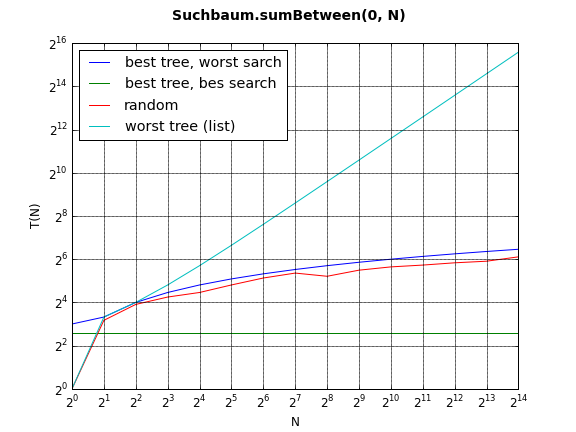
\includegraphics[width=\textwidth]{./IMG/plot.png}
    \caption[recur iter fast]{Aufwende der Suche in Abhängigkeit von der Baumstruktur und der geuschten Min und Max Werte, sowie der Anzahl der Knoten N}
\end{figure}
	
In Abbildung \ref{fig:plot} hat der \texttt{worst tree} eine lineare Komplexität $O(N)$, was auch auf die listenenartige Baumstruktur zurückzuführen ist. \texttt{best tree, best search} weißt eine Knostante Komplexität auf $O(1)$, nicht mehrmals die Schleife durchläuft, da die Wurzel das Ziel ist.
 \texttt{best tree, worst search} zeigt deutlich die Baumtiefe des Baumes wieder, da die Suche bis nach ganz unten bis zur letzten Ebene geht $O(log N)$.
 \texttt{random} weist auch eine Komplexität von $O(log N)$, sie liegt jedoch
unter der von \texttt{best tree, worst search}, da die Tiefe der einzelnen Zweige variiert und die Randzweige bei unserer Messung leider zu kurz kamen...

Es wurde die API des Quellcodes mit angehängt.

\end{document}
% vim: set spell spelllang=de :EOF
